% 2011 年湖北卷理科第 7 题：K 与并联的 A1、A2 组成的系统。
% 来源 PDF：普通高考/2011/2011湖北理.pdf，SHA-256 ba721f03ae90f88887c5cde27ae98dbea165d33c73e5ba45b4e4f56b0638b075。
% 原页：第 1 页第 1 栏上部，书页码 667。
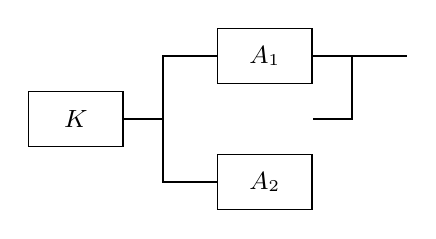
\begin{tikzpicture}[>=stealth, semithick, font=\small]
  \node[draw, minimum width=1.2cm, minimum height=0.7cm] (K) at (0,0) {$K$};
  \node[draw, minimum width=1.2cm, minimum height=0.7cm] (A1) at (2.4,0.8) {$A_1$};
  \node[draw, minimum width=1.2cm, minimum height=0.7cm] (A2) at (2.4,-0.8) {$A_2$};
  \draw (K.east) -- ++(0.5,0) coordinate (x) -- ++(0,0.8) -- (A1.west);
  \draw (x) -- ++(0,-0.8) -- (A2.west);
  \draw (A1.east) -- ++(0.5,0) coordinate (y) -- ++(0,-0.8) -- ++(-0.5,0);
  \draw (y) -- ++(0.7,0);
\end{tikzpicture}
